%\documentclass[compress,brown]{beamer}
\documentclass[compress,brown,xcolor=table]{beamer}

\usepackage{etex}
\mode<presentation>

\usetheme{metropolis} 

\hypersetup{pdfpagemode=FullScreen} % makes your presentation go automatically to full screen

% to have the same footer on all slides
%\setbeamertemplate{footline}[text line]{STUFF HERE!}
\setbeamertemplate{footline}[text line]{} % makes the footer EMPTY

% include packages
\usepackage{subfigure}
\usepackage{multicol}
\usepackage{amsmath}
\usepackage{epsfig}
\usepackage{graphicx}
\usepackage[all,knot]{xy}
\xyoption{arc}
\usepackage{url}
\usepackage{multimedia}
\usepackage{hyperref}

% Package pour le français
\usepackage[utf8]{inputenc}
\usepackage[french]{babel} % Pour adopter les règles de typographie française
\usepackage[T1]{fontenc} % Pour que LaTeX comprenne les caractères accentués ;
                         % norme iso-8859, cela risque de ne pas marcher avec
                         % des fichiers créés sous windows


     
%%%%%%%%%%%%%%%
%%%%%%%%%%%%%%%%%%%%%%%%%%%%%% Title Page Info %%%%%%%%%%%%%%%%%%%%%%%%%%%%%%%%%%%%%%%%%%%%

\title{Redes P2P y Bitcoin}
\author{Guillermo Galindo Ortuño \\ Carlos Santiago Sánchez Muñoz}
\institute{Fudamentos de Redes}
\date{}
%%%%%%%%%%%%%%%
%%%%%%%%%%%%%%%%%%%%%%%%%%%%%% Begin Your Document %%%%%%%%%%%%%%%%%%%%%%%%%%%%%%%%%%%%%%%


\begin{document}

%%%%%%%%%%%%%%%

\frame{
	\titlepage 
}

%%%%%%%%%%%%%%%

\frame{\tableofcontents}

%================================================================
\section{Redes P2P}
\begin{frame}{Definición}
P2P es una arquitectura de red que consiste en que cada nodo funciona
simultáneamente como cliente y como servidor.

Esta fue utilizada por aplicaciones como Napster, Spotify, Skype, etc.
\begin{figure}
		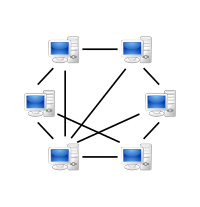
\includegraphics[width=5cm]{../images/p2pexample.png}
		\centering		
		\label{p4}
	\end{figure}

\end{frame}

\begin{frame}{Características}
	\begin{itemize}
	\item Escalabilidad
	\item Robustez
	\item Descentralización
	\item Distribución  de costes entre  los usuarios
	\item Anonimato
	\item Seguridad
\end{itemize}
	
\end{frame}

\begin{frame}{Clasificación}
	\begin{itemize}
	\item Redes desestructuradas
	\begin{figure}
		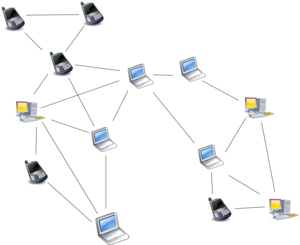
\includegraphics[width=2.7cm]{../images/Unstructured.png}
		\centering		
		\label{p4}
	\end{figure}
	\item Redes estructuradas
	\begin{figure}
		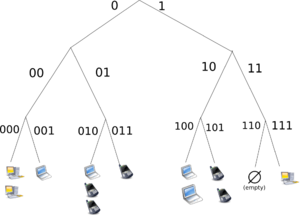
\includegraphics[width=2.7cm]{../images/Structured.png}
		\centering		
		\label{p4}
	\end{figure}
	\item Redes hibridas
	
\end{itemize}
\end{frame}
\begin{frame}{Problemas}
	\begin{itemize}
	\item Encontrar nodos ya conectados a la red
	\item Como se conectan los nodos sin IP entre ellos
\end{itemize}
\end{frame}

\section{Bitcoin}
\begin{frame}{Introducción}
	Bitcoin es una criptodivisa que utiliza un sistema totalemente
descentralizado. Se llama bitcoin tanto a la unidad monetaria y como al
protocolo y a la red que lo sustentan.\\

Ahora mismo un bitcoin esta valorado en aproximadamente 5000\$.
\end{frame}

\subsection{La cadena de bloques}
\frame{\sectionpage}

\begin{frame}{Bloques}
	Los bloques forman la cadena de bloques y almacenan un conjunto de transacciones. Estos poseen la siguiente estructura:
	\begin{figure}
		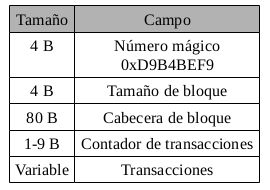
\includegraphics[width=6cm]{../images/blockstructure.png}
		\centering		
		\label{p4}
	\end{figure}

\end{frame}

\begin{frame}{Bloques}
	La cabecera de cada bloque posee la siguiente estructura:
	\begin{figure}
		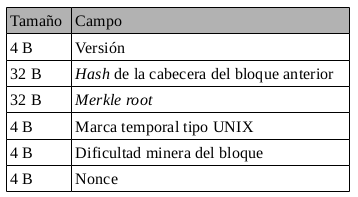
\includegraphics[width=7cm]{../images/headerstructure.png}
		\centering		
		\label{p4}
	\end{figure}
\end{frame}

\begin{frame}{Ejemplo cadena de bloques}
	Una cadena de bloques tendría una estructura similar a la mostrada abajo, y es gracias a esta estructura que resulta realmente complicado tratar de modificar un bloque ya validado para obtener beneficio ``ilegal'', ya que habría que volver a validar todos lo bloques que ``cuelguen de él''
	\begin{figure}[h]
	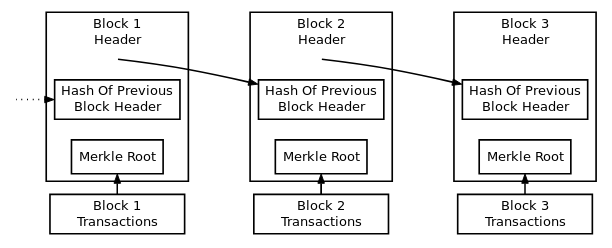
\includegraphics[width=10cm]{../images/blockchain.png}
	\centering		
	\label{p3}
\end{figure}

\end{frame}

\begin{frame}{Transacciones}
	Aunque pensemos que en las transacciones los satoshis van de una cartera a otra cartera, esto no es así, ya que las transacciones tienen salidas y entradas, y así ``viajan'' entre estas. 
	\begin{figure}[h]
	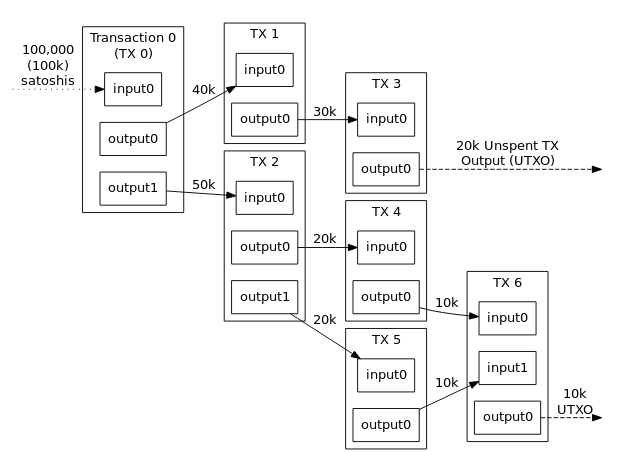
\includegraphics[width=8cm]{../images/transactions.png}
	\centering		
	\label{p3}
\end{figure}
\end{frame}

\begin{frame}{Transacciones: merkle tree y merkle root}
	Buscar si una transacción se encuentra en un bloque descargando el arbol entero de transacciones sería increíblemente costoso, por eso se utilizan los llamados ``merkle tree'' y ``merkle root''.
	Un ejemplo simplificado de un ``merkle tree'' sería el siguiente:
	\begin{figure}[h]
	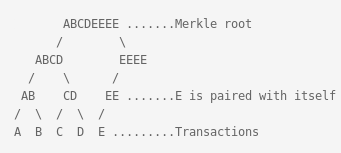
\includegraphics[width=7cm]{../images/merkleroot.png}
	\centering		
	\label{p5}
\end{figure}
\end{frame}

\begin{frame}{Prueba de trabajo}
	Validar un bloque en Bitcoin consiste a grandes rasgos en calcular un hash a partir de la cabecera de dicho bloque, y comprobar que el valor está por debajo de un umbral que es al que se llama "dificultad de validación". Esto es junto con la estructura de cadena es lo que realmente hace que sea dificil modificar las transacciones de bloques ya validados.
\end{frame}

\begin{frame}{Prueba de trabajo}
	Esta dificultad de validación se va modificando cada 2016 bloques validados en función del tiempo que hayan tardado en validarse estos bloques:
	\begin{itemize}
	\item Si ha tardado más de dos semanas, el valor que marca la dificultad se incrementa.
	\item Si ha tardado menos de dos semanas, el valor se decrementa.
\end{itemize}	
\end{frame}

\begin{frame}{Altura de bloque y forking}
	Llamamos altura de un bloque al número de bloques en la cadena entre este y el bloque génesis o bloque 0. Podría dar el caso en el que dos nodos validaran un bloque simultáneamente, lo que provocaría que hubiese dos bloques con la misma altura, lo que provocaría un aparente ``fork''.
\end{frame}

\begin{frame}{Altura de bloque y forking}
	Hay varios tipos de fork:
	\begin{figure}[h]
	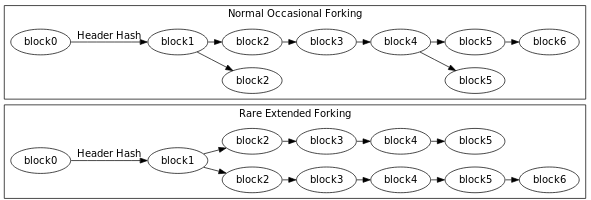
\includegraphics[width=10cm]{../images/forkingtypes.png}
	\centering		
	\label{p3}
	\end{figure}
El primero se da comúnmente, mientras que el segundo es raro que ocurra, pudiendo ocurrir a causa de un ataque del 51\%.
	
\end{frame}

\begin{frame}{Reglas de consenso}
	Para conseguir que todos los nodos tengan los mismos bloques en su mejor cadena existen las llamadas reglas de consenso. Estas son modificadas cada cierto tiempo, por lo que existen lapsos de tiempo en los que algunos nodos siguen las antiguas reglas y otros las nuevas, lo que puede ocasionar los siguientes problemas:
	
\end{frame}

\begin{frame}{Reglas de consenso}
	\begin{itemize}
	\item Un bloque que sea aceptado por las nuevas reglas no puede ser aceptado por las antiguas reglas. Esto produce un ``hardfork'' que tiene la siguiente forma:
\end{itemize}
	\begin{figure}[h]
	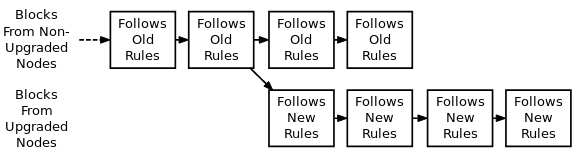
\includegraphics[width=10cm]{../images/hardforking1.png}
	\centering		
	\label{p3}
	\end{figure}
\end{frame}

\begin{frame}{Reglas de consenso}
	\begin{itemize}
	\item Un bloque no aceptado por las nuevas reglas es aceptado por las antiguas reglas(supuesto que los bloques aceptados por las nuevas reglas son aceptados por las antiguas).  Esto produce un ``softfork'' que tiene la siguiente forma:
\end{itemize}
	\begin{figure}[h]
	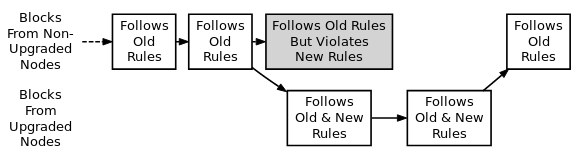
\includegraphics[width=10cm]{../images/softforking2.png}
	\centering		
	\label{p3}
	\end{figure}
\end{frame}

\subsection{Bitcoin como red P2P}
\frame{\sectionpage}

\begin{frame}
El protocolo de red Bitcoin permite que los nodos mantengan de forma colaborativa una red punto a punto para el intercambio de bloques y transacciones.

\begin{itemize}
	\item Los nodos completos descargan y verifican cada bloque y transacción antes de retransmitirlos a otros nodos.
	\item Los nodos de archivo almacenan toda la cadena de bloques y pueden servir bloques históricos a otros nodos.
	\item Los nodos podados son nodos completos que no almacenan toda la cadena de bloques.
\end{itemize}

\end{frame}

\begin{frame}{Descubriendo los nodos}
\begin{itemize}
	\item Cuando se inician por primera vez, los programas no conocen las direcciones IP de ninguno de los nodos completos activos.\\

	\item Para descubrir algunas direcciones IP, consultan uno o más nombres DNS que se encuentran en el código de los nodos.\\

	\item La respuesta a la búsqueda debe incluir uno o más registros DNS con direcciones IP de nodos completos que pueden aceptar nuevas conexiones entrantes.\\

	\item Las \textbf{semillas (seeds) DNS} son mantenidas por los miembros de la comunidad Bitcoin.
\end{itemize}
\end{frame}

\begin{frame}{Descubriendo los nodos}
\begin{itemize}
	\item Los programas no deben depender exclusivamente de semillas DNS. Un atacante malicioso en el medio puede devolver solo las direcciones IP de los nodos controlados por él, aislandolo.\\

	\item Una vez conectado a la red, sus nodos pueden comenzar a enviarle mensajes addr con direcciones IP y números de puerto -> Método completamente descentralizado de descubrimiento entre iguales.\\

	\item Los nodos a menudo abandonan la red o cambian sus direcciones IP, por lo que es los programas tienen que realizar varios intentos de conexión -> Retraso \\

	\item Para evitar este posible retraso, BitcoinJ siempre usa semillas dinámicas. Bitcoin Core trata de encontrar un equilibrio entre minimizar las demoras y evitar el uso innecesario de semillas DNS.
\end{itemize}
\end{frame}

\begin{frame}{Conectarse a los nodos}
\begin{itemize}
	\item La conexión se realiza enviando un mensaje con el número de versión, bloque y hora actual al nodo remoto.\\

	\item El nodo remoto responde con su propio mensaje de versión.\\

	\item Mensaje "verack".\\

	\item Ahora el cliente puede enviar al nodo remoto mensajes getaddr y addr para reunir nodos adicionales.\\
	
	\item Después de 90 min. el cliente asumirá que la conexión se ha cerrado.\\
\end{itemize}
\end{frame}

\begin{frame}{Descarga del bloque inicial}
\textbf{¿Qué es descargar el IBD?}\\
\begin{itemize}
	\item Antes de que un nodo completo pueda validar transacciones debe descargar y validar todos los bloques desde el 1 hasta la punta actual de la mejor cadena de bloques.\\

	\item Es reutilizable cada vez que se quiera hacer una descarga de un numero considerable de bloques.\\

	\item Bitcoin Core usa el método IBD cada vez que el último bloque en su cadena de tiene un tiempo de cabecera de bloque de más de 24 horas o si su cadena de bloque local está 144 bloques más baja que su cadena de encabezado local.\\
\end{itemize}
\end{frame}

\begin{frame}{Headers-First}
Bitcoin Core 0.10.0 usa un método de descarga de bloque inicial (IBD) llamado "Headers-first". El objetivo es descargar las cabeceras para la mejor cadena de cabeceras, validarlos parcialmente lo mejor posible y luego descargar los bloques correspondientes en paralelo.\\

\begin{figure}[h]
	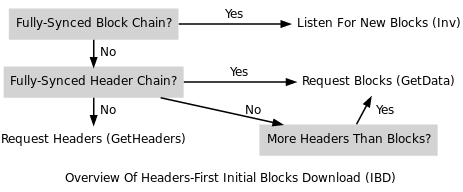
\includegraphics[width=9cm]{../images/Image1.png}
	\centering		
\end{figure}

\end{frame}

\begin{frame}{Headers-First}
La primera vez que se inicia un nodo tiene un bloque en su cadena de mejor bloque local: el bloque genesis codificado (bloque 0). El nodo elige un nodo remoto, que llamaremos nodo de sincronización, y le envía el mensaje ``getheader'':\\

\begin{figure}[h]
	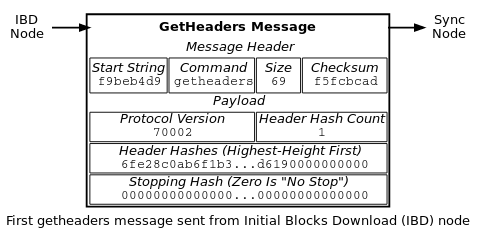
\includegraphics[width=10cm]{../images/Image2.png}
	\centering		
	\caption{GetHeaders Message}
	\label{p5}
\end{figure}
\end{frame}

\begin{frame}{Headers-First}
\begin{itemize}
	\item En el campo de hash de cabecera del mensaje ``getheaders'', el nuevo nodo envía el hash de encabezado del único bloque que tiene, el bloque de generación (6fe2 ... 0000). También establece el campo de parada de hash en todos los ceros para solicitar una respuesta de tamaño máximo.\\

	\item El nodo de sincronización toma el primer hash de encabezado y busca en su mejor cadena de bloque local un bloque con ese hash. Encuentra que el bloque 0 coincide, por lo que responde con un 2.000 cabeceras a partir del bloque 1.
\end{itemize}
\end{frame}

\begin{frame}{Headers-First}
Los hashes de estas cabeceras los manda en el mensaje mostrado a continuación:\\
\begin{figure}[h]
	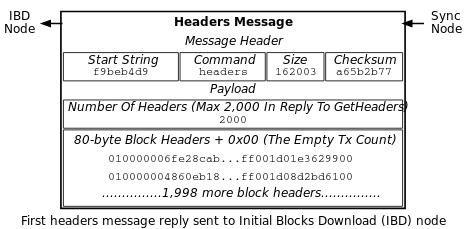
\includegraphics[width=10cm]{../images/Image3.png}
	\centering		
	\caption{Headers Message}
	\label{p5}
\end{figure}
\end{frame}

\begin{frame}{Headers-First}
El nodo IBD puede validar parcialmente estos encabezados.\\

Una vez validados parcialmente los encabezados se pueden hacer dos cosas en paralelo:

\begin{enumerate}
	\item \textbf{Descargar más encabezados:} el nodo IBD puede enviar otro "getheaders".\\

	\item \textbf{Descargar bloques:} mientras el nodo IBD continúa descargando cabeceras, y después de que terminen de descargarse, el nodo IBD solicitará y descargará cada bloque.
\end{enumerate}

Bitcoin Core solicitará un máximo de 128 bloques simultáneamente.
\end{frame}

\begin{frame}{Emisión de bloques}
Cuando un minero descubre un nuevo bloque, transmite el nuevo bloque a sus nodos conectados

\begin{itemize}

	\item \textbf{Unsolicited Block Push:} el minero envía un mensaje de bloque a cada uno de sus peers completos con el nuevo bloque.\\

	\item \textbf{Standard Block Relay:} el minero, que actúa como un nodo de retransmisor estándar, envía un mensaje \```inv'' a cada uno de sus nodos conectados con un inventario que hace referencia al nuevo bloque.\\

	\item \textbf{Direct Headers Announcement:} un nodo retransmisor puede omitir la sobrecarga de ida y vuelta de un mensaje \```inv'' seguido de encabezados obsoletos mediante el envio de un mensaje de encabezado.

\end{itemize}

Por defecto, Bitcoin Core difunde bloques con la 3ª política a todos los nodos que han enviado señales con ``sendheaders'' y la 2ª a los otros.
\end{frame}

\begin{frame}{Bloques huérfanos}
Bloques cuyo campo hash de encabezado del bloque anterior hace referencia a un encabezado de bloque que este nodo aún no ha visto, es decir, no tienen padres conocidos.\\

\begin{figure}[h]
	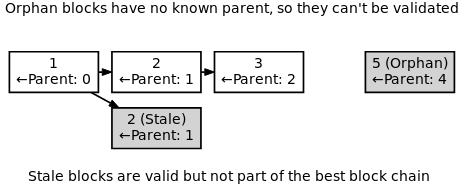
\includegraphics[width=9cm]{../images/Image4.png}
	\centering		
	\label{p5}
\end{figure}
\end{frame}

\begin{frame}{Memory pool}

\begin{itemize}
	\item Debido a que las transacciones no confirmadas no tienen un estado permanente en Bitcoin, se almacenan en memoria no persistente, llamándolas ``memory pool''.
	
	\item Cuando un par se apaga, su ``memory pool'' se pierde a excepción de cualquier transacción almacenada por su billetera ("wallet").\\

	\item Las transacciones que se extraen en bloques que luego se vuelven obsoletos se pueden volver a agregar a ``memory pool''.\\

	\item Bitcoin Core elimina los bloques obsoletos de la cadena uno por uno, comenzando con la punta (bloque más alto).
\end{itemize}

\end{frame}

\begin{frame}{Nodos con mal comportamiento}
\begin{itemize}
	\item Existen mecanismos para castigar a los nodos que toman ancho de banda y recursos informáticos mediante el envío de información falsa.

	\item Si un peer obtiene un banscore por encima del umbral ($-banscore = <n>$), estará prohibido durante el número de segundos definidos por $-bantime = <n>$, que es 86400s=24h.
\end{itemize}
\end{frame}

\subsection{Minado}
\frame{\sectionpage}

\begin{frame}
La minería agrega nuevos bloques a la cadena de bloques, por lo que es difícil modificar el historial de transacciones. Toma dos formas:
\begin{itemize}
	\item Minería en solitario.
	\item Minería combinada.
\end{itemize}
\end{frame}

\begin{frame}{Minería en solitario}
\begin{itemize}
	\item El minero intenta generar nuevos bloques por su cuenta, donde genera ganancias a partir del "premio" por bloque y de las tasas por transacción.\\

	\item Usan ``bitcoind" para obtener nuevas transacciones de la red. Su software de minería solicita periódicamente nuevas transacciones utilizando el RPC ``getblocktemplate".\\
\end{itemize}
\end{frame}

\begin{frame}{Minería en solitario}
\begin{itemize}
\item El software de minería construye un bloque usando una plantilla y crea un encabezado de bloque.

\item Se envía el encabezado del bloque a su hardware de minería (un ASIC). El hardware de minería itera a través de cada valor posible para el encabezado del bloque y genera el hash correspondiente.
\end{itemize}

\begin{figure}[h]
	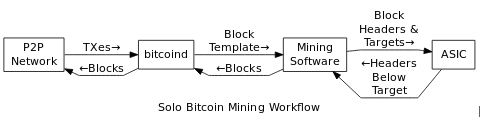
\includegraphics[width=11cm]{../images/Image5.png}
	\centering		
	\label{p5}
\end{figure}

\end{frame}

\begin{frame}{Minería combinada}
\begin{itemize}
	\item El minero reúne recursos con otros mineros para encontrar bloques más a menudo, con los beneficios compartidos entre los mineros en una correlación aproximada con la cantidad de potencia de hashing que aportaron.\\

	\item El software de minería de cada minero se conecta al grupo y solicita la información que necesita para construir encabezados de bloque.\\

	\item El minero envía al grupo una copia de la información que el grupo necesita para validar que el encabezado tiene un hash debajo del objetivo y que el bloque de transacciones es válido.\\
\end{itemize}
\end{frame}

\begin{frame}{Minería combinada}

\begin{itemize}
	\item La información que el minero envía al grupo se denomina participación.
	\item Las tarifas de recompensa y transacción del bloque se pagan al grupo de minería.
	\item El grupo minero paga una parte de estos ingresos a mineros.
\end{itemize}

\begin{figure}[h]
	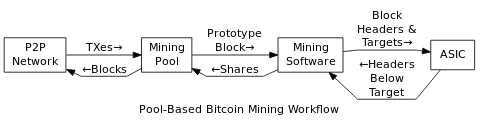
\includegraphics[width=10cm]{../images/Image6.png}
	\centering		
\end{figure}

\end{frame}

\subsection{Demo de una cadena de bloques}
\frame{\sectionpage}

\begin{frame}{Demo}
	El archivo fuente de la cadena de bloques se encuentra en https://	github.com/guillegalor/P2P\_BITCOIN/blockchain.py
\end{frame}

\begin{frame}{Demo}
	Para interactuar con la cadena lo haremos a traves de mensajes http, y en concreto usando curl. Los mensajes para interactuar con ella son los siguiente:
	\begin{itemize}
	\item curl -X POST -H "Content-Type: application/json" -d '$\{$
 "sender": "...",\\
 "recipient": "...",\\
 "amount": n\\
$\}$' "http://localhost:5000/transactions/new"
	\item curl "http://localhost:5000/mine"
	\item curl "http://localhost:5000/chain"
		
\end{itemize}
\end{frame}

\begin{frame}{Demo}
	\begin{itemize}
	\item curl -X POST -H "Content-Type: application/json" -d '$\{$\\
                                     "nodes" : ["http://localhost:5000/"]\\
                                    $\}$' "http://localhost:500/nodes/register"
    \item curl "http://localhost:5000/nodes/resolve"                                	

	
\end{itemize}
\end{frame}
\begin{frame}{Agradecimientos}
	\begin{itemize}
	\item Daniel van Flymen, @dvf\\
	https://github.com/dvf/blockchain --- Repositorio original con la cadena de bloques\\
	https://blockchain.works-hub.com/blog/Learn-Blockchains-by-Building-One --- Articulo donde explica el codigo completo
	\item Daniel Pozo Escalona, @danipozo
	

\end{itemize}
\end{frame}

\section{Bibliografía}

\begin{frame}{Bibliografía}
\begin{itemize}
	\item https://es.wikipedia.org/wiki/Peer-to-peer
	\item https://es.wikipedia.org/wiki/P2P\_privado
	\item https://es.wikipedia.org/wiki/Friend-to-friend
	\item https://es.wikipedia.org/wiki/Bitcoin
	\item https://en.wikipedia.org/wiki/Bitcoin\_network
	\item www.deic.uab.cat/~cperez/papers/FC2014-donet-perez-herrera.pdf
	\item https://bandaancha.eu/foros/todos-programas-p2p-aqui-839441
	\item https://es.wikipedia.org/wiki/Bitcoin
	\item https://en.wikipedia.org/wiki/Bitcoin
	\item https://www.bitcoin.com/
	\item https://en.bitcoin.it/wiki/
\end{itemize}
\end{frame}


\end{document}

